%  \documentclass[conference]{IEEEtran}
% \documentclass[a4paper]{IEEEtran}
\documentclass[a4paper, conference]{IEEEtran}
\IEEEoverridecommandlockouts
\pdfminorversion=6
% The preceding line is only needed to identify funding in the first footnote. If that is unneeded, please comment it out.
\usepackage{epsfig}
\usepackage{svg}
\usepackage{cite}
\usepackage{amsmath,amssymb,amsfonts}
\usepackage{mathtools}
\usepackage{amsthm}
\newtheorem{definition}{Definition}
%\usepackage{algorithmic}
%\pagenumbering{gobble}
\usepackage{graphicx}
\usepackage{textcomp}
\usepackage{xcolor}
\usepackage{array}
\usepackage{listings}
\usepackage{multirow}
\usepackage{multicol}

\usepackage[T1]{fontenc}
\usepackage{enumitem}

\usepackage{array}
%\usepackage{lipsum}
%\usepackage{multirow}
%\usepackage{enumitem}
\usepackage[utf8]{inputenc}
\usepackage[noend]{algpseudocode}
\usepackage{pseudocode}
\usepackage[linesnumbered,ruled,vlined]{algorithm2e}
\usepackage{balance}
\usepackage{caption}
\usepackage{comment}
\usepackage{tikz}
\usetikzlibrary{positioning,shapes.geometric}


\algnewcommand{\IfThenElse}[3]{% \IfThenElse{<if>}{<then>}{<else>}
	\State \algorithmicif\ #1\ \algorithmicthen\ #2\ \algorithmicelse\ #3}

% custom macro definitions

%\include{resource/header-codelisting} % not present in this repo -- listings used directly below
\newcolumntype{P}[1]{>{\centering\arraybackslash}p{#1}}
\newcolumntype{M}[1]{>{\centering\arraybackslash}m{#1}}

%duclm: tikz for drawing LTS
%\include{resource/tikzdrawings}
% Algorithm
%\usepackage{epsfig}
\usepackage[linesnumbered,ruled,vlined]{algorithm2e}
%\makeatletter
%\def\BState{\State\hskip-\ALG@thistlm}
%\makeatother

%\usepackage[top=0.75in,bottom=0.75in,left=1in,right=1in,]{geometry}
%\usepackage{listings}

%\pagestyle{plain} % removes running headers

% custom macro definitions
%\include{resource/header}

%\include{resource/header-javacodelisting}
%\breakauthorline{}% breaks lines after the n-th author
% % % % % % % % % %
% % % % % % % % % %
% CUSTOM CONFIGURATIONS:
% graphics
\graphicspath{ {images/} }
\DeclareGraphicsExtensions{.png,.jpg,.eps,.pdf}
\usepackage{}
% % % % % % % % % %

\def\BibTeX{{\rm B\kern-.05em{\sc i\kern-.025em b}\kern-.08em
		T\kern-.1667em\lower.7ex\hbox{E}\kern-.125emX}}

\newcommand{\hdfigure}[3]{%
	\begin{figure}[phtb]%
		\vspace{-1ex}%
		\begin{center}%
			\includegraphics[scale=#2]{#1}%
			\vspace{-1ex}%
			\caption{#3\label{fig:#1}}%
		\end{center}%
		\vspace{-3ex}%
\end{figure}}

\newcommand{\hdfigurestar}[3]{%
	\begin{figure*}[phtb]%
		\vspace*{-1ex}%
		\begin{center}%
			\includegraphics[scale=#2]{#1}%
			\vspace*{-1ex}%
			\caption{#3\label{fig:#1}}%
		\end{center}%
		\vspace*{-3ex}%
\end{figure*}}

\newcommand{\hdfigurerot}[3]{%
	\begin{figure}[phtb]%
		% \vspace*{2ex}%
		\begin{center}%
			% \vspace*{-30ex}%
			\includegraphics[angle=90,origin=B,scale=#2]{#1}%
			% \vspace*{-6ex}%
			\caption{#3\label{fig:#1}}%
			% \vspace*{-18ex}%
		\end{center}%
\end{figure}}

%%%%%%%%%%%%%%%%%%%%%%%%%%%%%%%%%%%%%%%%%%%%%%
\begin{document}

\title{
\huge Checking the Conformance between Goal Models \\
and Process Models Based on Scenario Synchronization
%{\footnotesize \textsuperscript{*}Note: Sub-titles are not captured in Xplore and
%should not be used}
%\thanks{Identify applicable funding agency here. If none, delete this.}
}

\author{
    \IEEEauthorblockN{
        Duc-Quyen Nguyen, Minh-Phuc Hoang, and Huy-Hung Dao, Duc-Hanh Dang
    }\IEEEauthorblockA{
	University of Engineering and Technology, Vietnam National University, Hanoi\\
     % NOTE: only "hanhdd" is a confirmed address (reused from the co-author's known VNU
     % account); the other three are placeholders and MUST be replaced with the real
     % student/account IDs before submission.
     Email: {\tt\{TODO-quyen|TODO-phuc|TODO-hung|hanhdd\}@vnu.edu.vn}
     }
}

\pagestyle{empty}
\maketitle
\thispagestyle{plain} %--to make title page number less
\pagestyle{plain}    % -- to make other pages number less.
%\thispagestyle{empty}
%%%%%%%%%%%%%%%%%%%%%%%%%%%%%%%%%%%%%%%%%%%%%%
\begin{abstract}
Model-driven engineering often represents a system's intentions and operational behavior in separate but complementary goal and process models. Keeping these views consistent is difficult because they use different abstractions, evolve independently, and do not necessarily share the system state needed to interpret an execution. Building on scenario synchronization, we propose ACL as a shared state model: process executions update ACL states, while goal models evaluate their intentions over the same states. We instantiate the methodology with extended i* and simplified BPMN semantics, check their consistency along checkpoint traces, and translate the integrated models to Event-B for Rodin verification. In the \textit{MeetingScheduler} case study, the USE checker identifies a completed BPMN trace that leaves the root i* goal unsatisfied for an omitted participant, while the generated Event-B development passes Rodin static checking and discharges all 126 proof obligations. The \textit{Incident Response} case study executes through the same pipeline without modification, providing further evidence that the shared-state method applies across distinct process scenarios.
\end{abstract}
%%%%%%%%%%%%%%%%%%%%%%%%%%%%%%%%%%%%%%%%%%%%%%
\begin{IEEEkeywords}
	GORE; i*; BPMN; MDE; UML/OCL; Conformance Checking;
\end{IEEEkeywords}
% \vspace{-1em}
%%%%%%%%%%%%%%%%%%%%%%%%%%%%%%%%%%%%%%%%%%%%%%
\section{Introduction}
\label{sect:intro}
%%%%%%%%%%%%%%%%%%%%%%%%%%%%%%%%%%%%%%%%%%%%%%

Model-driven engineering (MDE) places models at the center of the software engineering process and treats them as first-class engineering artifacts. Within MDE, a system is often described by multiple complementary models that capture different concerns and levels of abstraction. Goal models represent stakeholders, intentions, and rationale, thereby explaining \emph{why} a system is needed, whereas process models describe activities, responsibilities, and execution order, thereby explaining \emph{how} those intentions are operationalized~\cite{gobis2015}. The intentions expressed in a goal model are expected to be realized by the behavior described in the corresponding process model. Establishing and maintaining consistency between the two models provides traceability from goals to their process-level realization and supports the detection of divergence as the models evolve~\cite{gobis2015,caballero2026alig}.

Checking consistency between goal and process models is challenging for several reasons. First, the two types of models are developed at different levels of abstraction: one goal may be realized by multiple activities, while one activity may contribute to several goals~\cite{groner2014vadl,caballero2026alig}. Second, they are often developed independently, at different stages and by different roles, making manually established correspondences costly and prone to divergence as the models change~\cite{gobis2015,groner2014vadl}. Moreover, consistency may depend not only on model-level elements but also on the concrete instances involved in an execution. Multiple runtime instances may be represented by the same actor, role, or activity, yet reach different states and consequently yield different goal-satisfaction outcomes.

Existing approaches employ different mechanisms for checking consistency. GoBIS supports integration and traceability between the two views at design time~\cite{gobis2015}; Gr"oner et al. formalize correspondences using Description Logics to detect inconsistencies~\cite{groner2014vadl}; and Caballero-Villalobos et al. translate the two models into transition systems and evaluate goal satisfaction over synchronized executions~\cite{caballero2026alig}. Despite their different reasoning mechanisms, these approaches rely on correspondences established in advance between the two models, which must also be maintained as the models evolve independently.
In our previous work, models at different abstraction levels were synchronized through a shared conceptual model represented in UML, while OCL was used to specify and check consistency conditions over synchronized states~\cite{dang2010jucs}. However, for the goal--process setting, this UML/OCL representation does not explicitly capture the organizational context required to interpret intentions.

Building on this foundation, we propose ACL as an intermediate language for representing the shared organizational and domain state of goal and process models. ACL extends the shared-state principle of our previous work by explicitly representing domain entities, organizational concepts, and their runtime instances. In our approach, process execution updates the ACL state, while the goal model evaluates intention satisfaction over the same state, thereby distinguishing different instances represented by the same model element.

To interpret i* and BPMN over ACL, we adapt the two languages only where necessary and use OCL as a common expression language over the shared state. OCL specifies conditions of intentional elements in i* and guards, preconditions, and postconditions in BPMN. ACL, i*, and BPMN are thus given a unified state-based semantics: ACL represents the system state, BPMN describes how that state evolves, and i* specifies the intentions evaluated over that state.

We also define systematic transformation rules from the unified semantics of ACL, i*, and BPMN into an integrated Event-B model. These rules preserve the relationships among the three models, allowing their shared semantics to be represented and formally checked in Rodin through static checking and proof obligations.

In the \textit{MeetingScheduler} case study, the approach detects a completed BPMN execution in which an applicable i* root goal remains unsatisfied for a particular participant. The generated Event-B model passes Rodin static checking and discharges all 126 proof obligations. The \textit{Incident Response} case study applies the same approach without requiring changes to the processing pipeline.

This paper makes three main contributions: i) ACL, an intermediate shared-state language for goal and process models; ii) a unified state-based semantics for ACL, i*, and BPMN, with OCL serving as the common expression language over the shared state; and iii) transformation rules from this unified semantics to Event-B to support formal checking in Rodin. The approach is implemented in a USE prototype and illustrated through the case studies.

The remainder of this paper is organized as follows. Section~\ref{sect:motivation} presents the motivating example. Section~\ref{sect:overview} provides an overview of the approach, including the metamodels, their semantics, and the checking mechanism. Section~\ref{sect:toolSupport} describes the tool support. Section~\ref{sect:evaluative} presents the research questions and evaluates the approach against related techniques. Section~\ref{sect:discussion} discusses trade-offs and limitations. Section~\ref{sect:relatedWork} reviews related work. Finally, Section~\ref{sect:conclusion} concludes the paper.



%%%%%%%%%%%%%%%%%%%%%%%%%%%%%%%%%%%%%%%%%%%%%%
\section{Motivating Example}
\label{sect:motivation}
%%%%%%%%%%%%%%%%%%%%%%%%%%%%%%%%%%%%%%%%%%%%%%

\label{subsect:umlocl}

Consider \textit{ProposalReview}, a proposal-handling scenario involving a
\textit{Proposal Manager} and a \textit{Customer}. The i* model captures the
intentions that should be achieved, whereas the BPMN model describes the
activities used to process the proposal.

Figure~\ref{fig:istar-proposal-review} presents the intentional view. The root goal
\texttt{Proposal completed} requires the proposal to be ready for
finalization and then finalized and sent. In turn, readiness requires that
the current proposal is prepared and validated, that the customer review has
been received, and that any customer feedback has been resolved. If changes
are requested, they must therefore be incorporated without losing the
validation required for the proposal currently being processed. In other
words, validation concerns the current proposal revision, rather than merely
the fact that a validation task has occurred.

\begin{figure}[htbp]
\vspace{-.3em}
\begin{center}
\includegraphics[width=\columnwidth,keepaspectratio]{images/proposal_review_istar.jpg}
\vspace{-1.1em}
\begin{center}
\caption{i* model of \textit{ProposalReview}.}
\label{fig:istar-proposal-review}
\end{center}
\vspace{-2.7em}
\end{center}
\end{figure}


% ===============================================================
% ==== MUST BE DELETED LATER ON, REPLACED BY PROPOSAL REVIEW ====
% ===============================================================

\begin{figure}[htbp]
\vspace{-.3em}
\begin{center}
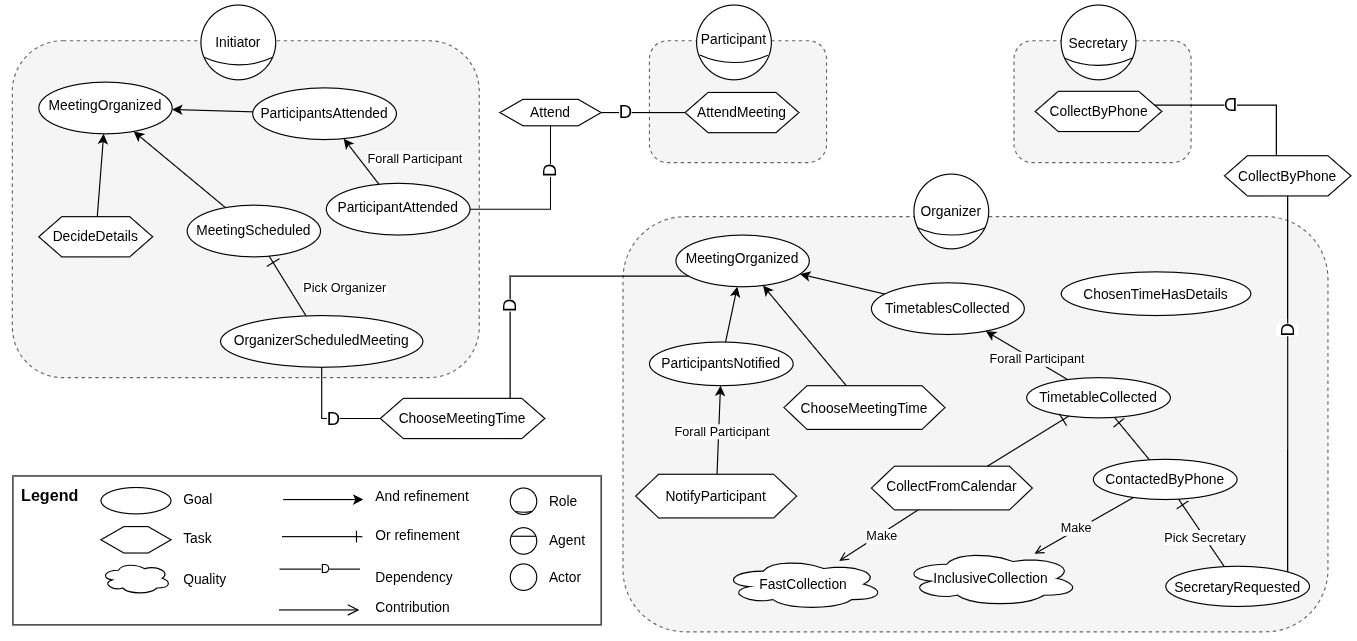
\includegraphics[width=\columnwidth,keepaspectratio]{images/Istarmodel.png}
\vspace{-1.1em}
\begin{center}
\caption{i* model of \textit{MeetingScheduler}.}
\label{fig:istar-mtg}
\end{center}
\vspace{-2.7em}
\end{center}
\end{figure}

The corresponding operational view is shown in
Figure~\ref{fig:bpmn-proposal-review}. The proposal is first prepared and validated
and is then reviewed by the customer. If the customer requests changes,
\texttt{Update proposal} is executed before the process proceeds to
\texttt{Finalize proposal} and \texttt{Send proposal}. At the model level, these activities appear to provide a complete operational realization of the intentions expressed in the i* model, and the process can proceed normally to completion.

\begin{figure}[htbp]
\vspace{-.3em}
\begin{center}
\includegraphics[width=\columnwidth,keepaspectratio]{images/proposal_review_bpmn_with_legend.jpg}
\vspace{-1.1em}
\begin{center}
\caption{BPMN model of \textit{ProposalReview}.}
\label{fig:bpmn-proposal-review}
\end{center}
\vspace{-2.7em}
\end{center}
\end{figure}


% ===============================================================
% ==== MUST BE DELETED LATER ON, REPLACED BY PROPOSAL REVIEW ====
% ===============================================================
\begin{figure}[htbp]
\vspace{-.3em}
\begin{center}
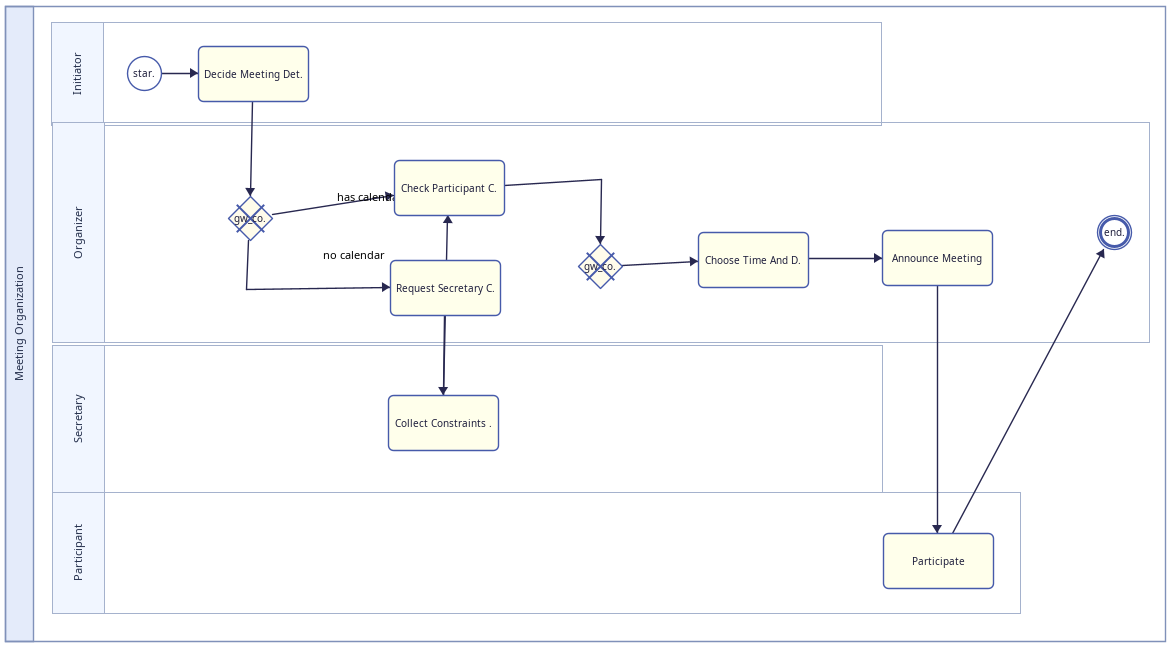
\includegraphics[width=\columnwidth,keepaspectratio]{images/BPMNmodel.png}
\vspace{-1.1em}
\begin{center}
\caption{BPMN model of \textit{MeetingScheduler}.}
\label{fig:bpmn-mtg}
\end{center}
\vspace{-2.7em}
\end{center}
\end{figure}

This apparent consistency, however, does not necessarily hold when the effects of these activities are interpreted over the evolving shared state. Semantically, a proposal is ready for completion only if the proposal currently being processed has been validated. After \texttt{Validate proposal}, this condition holds. However, when \texttt{Update proposal} modifies the proposal in response to customer feedback, the current proposal changes while its validation does not. The previously established validation condition therefore no longer holds. The BPMN control flow can nevertheless continue through \texttt{Finalize proposal} and \texttt{Send proposal} and reach the end event. Thus, the process completes successfully at the control-flow level, while the resulting state does not satisfy the intention that the current proposal must be validated.

The resulting mismatch reveals a limitation of static goal--process correspondences. The
mapping may correctly associate \texttt{Validate proposal} with the goal that
the proposal is validated, and \texttt{Update proposal} with the goal that
requested changes are incorporated. However, these mappings only describe how
individual activities contribute to individual goals. They do not capture how
the effect of one activity may undo a condition established by an earlier
activity. In this example, \texttt{Update proposal} changes the current
proposal revision and therefore invalidates the validation established before
the update. Detecting such an inconsistency requires both process effects and
goal conditions to be interpreted over the same evolving state.

%%%%%%%%%%%%%%%%%%%%%%%%%%%%%%%%%%%%%%%%%%%%%%%%%%%%%%%%%%%%%%%%%%%%%
\section{Overview of Our Approach}
\label{sect:overview}
%%%%%%%%%%%%%%%%%%%%%%%%%%%%%%%%%%%%%%%%%%%%%%%%%%%%%%%%%%%%%%%%%%%%%

The proposed method brings ACL, BPMN, and i* into one state-based verification workflow around a single principle: process execution and goal evaluation share the same runtime state. ACL makes this state explicit by representing domain objects and organizational instances; BPMN execution progresses over a control-flow configuration and constrains how the ACL state may change; and i* intentional elements are evaluated over the resulting ACL states rather than over an independent representation of the environment. OCL is the common expression language over this shared state throughout: ACL invariants characterize admissible states, BPMN preconditions and postconditions constrain execution, and intentional conditions determine goal satisfaction. What follows is not a complete formal semantics of ACL, BPMN, i*, and OCL, but only the elements needed to state precisely how a process execution relates to goal satisfaction: Section~\ref{sec:acl-language} defines the shared ACL state, Section~\ref{sec:bpmn} the BPMN control state and its ACL-facing contracts, Section~\ref{sec:istar} instance-level goal evaluation over that state, Section~\ref{sec:eventb-transformation} their joint transformation to Event-B, and Section~\ref{sec:checking} the resulting synchronization and scenario-conformance criterion.

The method receives three model specifications and a scenario specification; the latter supplies an initial ACL population, the concrete process instance and execution choices, and, optionally, expected i* markings used as an oracle. Figure~\ref{fig:overview} summarizes the resulting workflow. First, the three models are compiled and cross-referenced: a BPMN pool is bound to an ACL group, BPMN lanes and i* actors are bound to ACL roles, and all OCL expressions are type-checked over the ACL schema. Second, an AOL snapshot instantiates the initial ACL state $\sigma_M^0$. Third, the selected BPMN scenario is executed from $\sigma_M^0$ as a sequence of synchronized steps (Section~\ref{sec:checking}), and every resulting state is retained as a checkpoint at which the i* semantics evaluates the applicable goal and task occurrences and propagates their markings through refinements and dependencies. Finally, the checker combines ACL validity, BPMN execution, root-goal satisfaction, and the optional oracle into one conformance verdict and a diagnostic trace. In parallel, the ACL, BPMN, and i* specifications are transformed into one Event-B development whose proof obligations are discharged in Rodin: the execution branch answers whether the selected scenario conforms, while the Event-B branch checks that the integrated formalization is itself well-defined and preserves its stated invariants.

\begin{figure}[htbp]
\vspace{-.3em}
\begin{center}
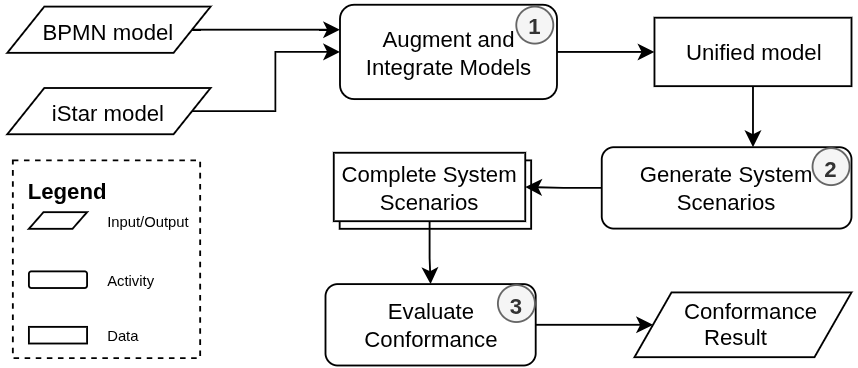
\includegraphics[width=\columnwidth,keepaspectratio]{images/overview.png}
\vspace{-1.1em}
\begin{center}
\caption{Overview of the proposed approach.}
\label{fig:overview}
\end{center}
\vspace{-2.7em}
\end{center}
\end{figure}

%%%%%%%%%%%%%%%%%%%%%%%%%%%%%%%%%%%%%%%
\subsection{The ACL Language}
\label{sec:acl-language}
%%%%%%%%%%%%%%%%%%%%%%%%%%%%%%%%%%%%%%%

ACL is a structural language for specifying the organizational and domain state shared by the process and goal views. Rather than a general-purpose class diagram, an ACL specification reads like a small declarative language: a \emph{group} declaration directly contains the \emph{role} declarations and nested \emph{group} declarations that belong to it, together with the group's own properties, as illustrated by the excerpt in Figure~\ref{fig:acl-metamodel}. An \emph{entity} instead represents a domain object that relates to this organizational structure only through an ordinary association, never through containment. Every role, group, or entity may own typed properties, and associations, aggregations, and compositions relate their occurrences with multiplicities declared at both ends. Role extension is an organizational chain rather than a class hierarchy: an occurrence of a child role is played through exactly one occurrence of its parent role, and the resulting chain terminates at one agent. Compatibility is declared for a pair of roles within a group; undeclared role pairs conflict by default. These constructs retain the organizational concepts of role and group used in MOISE~\cite{hubner2002moise}, expressed here as containment-based declarations and given the domain state and OCL-checked constraints needed to evaluate goals and process guards.

\begin{figure}[htbp]
\vspace{-.3em}
\begin{center}
\resizebox{\columnwidth}{!}{%
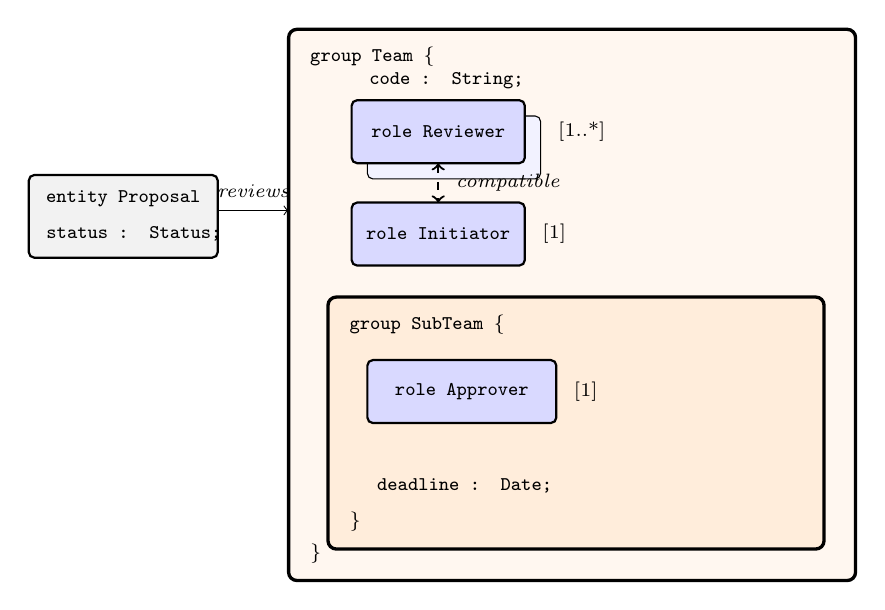
\begin{tikzpicture}
% entity box, outside the containment tree
\draw[rounded corners=2pt, thick, fill=black!5] (-3.3,-0.5) rectangle (-0.9,0.55);
\node[font=\ttfamily\bfseries\scriptsize] at (-2.1,0.25) {entity Proposal};
\node[anchor=west, font=\ttfamily\scriptsize] at (-3.2,-0.2) {status : Status;};
% association crossing into the group (not containment)
\draw[->, thin] (-0.9,0.1) -- (0.0,0.1);
\node[font=\scriptsize\itshape] at (-0.45,0.35) {reviews};
% outer group box: Team
\draw[very thick, rounded corners=3pt, fill=orange!6] (0.0,-4.6) rectangle (7.2,2.4);
\node[anchor=north west, font=\ttfamily\bfseries\scriptsize] at (0.15,2.3) {group Team \{};
\node[anchor=west, font=\ttfamily\scriptsize] at (0.9,1.75) {code : String;};
\node[anchor=south west, font=\ttfamily\bfseries\scriptsize] at (0.15,-4.5) {\}};
% role box: Reviewer, shadow stack denotes [1..*]
\draw[rounded corners=2pt, fill=blue!5] (1.0,0.5) rectangle (3.2,1.3);
\draw[rounded corners=2pt, thick, fill=blue!15] (0.8,0.7) rectangle (3.0,1.5);
\node[font=\ttfamily\scriptsize] at (1.9,1.1) {role Reviewer};
\node[anchor=west, font=\scriptsize] at (3.3,1.1) {[1..*]};
% role box: Initiator
\draw[rounded corners=2pt, thick, fill=blue!15] (0.8,-0.6) rectangle (3.0,0.2);
\node[font=\ttfamily\scriptsize] at (1.9,-0.2) {role Initiator};
\node[anchor=west, font=\scriptsize] at (3.1,-0.2) {[1]};
% compatibility link between the two roles
\draw[<->, dashed, thick] (1.9,0.7) -- (1.9,0.2);
\node[anchor=west, font=\scriptsize\itshape] at (2.0,0.45) {compatible};
% nested group box: SubTeam, contained inside Team
\draw[very thick, rounded corners=3pt, fill=orange!14] (0.5,-4.2) rectangle (6.8,-1.0);
\node[anchor=north west, font=\ttfamily\bfseries\scriptsize] at (0.65,-1.1) {group SubTeam \{};
\node[anchor=south west, font=\ttfamily\bfseries\scriptsize] at (0.65,-4.1) {\}};
% role box: Approver, contained inside SubTeam
\draw[rounded corners=2pt, thick, fill=blue!15] (1.0,-2.6) rectangle (3.4,-1.8);
\node[font=\ttfamily\scriptsize] at (2.2,-2.2) {role Approver};
\node[anchor=west, font=\scriptsize] at (3.5,-2.2) {[1]};
\node[anchor=west, font=\ttfamily\scriptsize] at (1.0,-3.4) {deadline : Date;};
\end{tikzpicture}%
}
\vspace{-1.1em}
\begin{center}
\caption{The ACL language as declarative, block-structured syntax rather than a class hierarchy. Solid nesting is containment: \texttt{group Team} directly encloses its \texttt{role} members and a nested \texttt{group SubTeam}, which in turn encloses its own role. A thin arrow is an ordinary domain association crossing from an \texttt{entity} into the containment tree; a dashed double arrow is a declared role \texttt{compatible} constraint.}
\label{fig:acl-metamodel}
\end{center}
\vspace{-2.7em}
\end{center}
\end{figure}

An ACL specification is a schema; Definition~\ref{def:acl-model} makes precise the state space it admits.

\begin{definition}[ACL Model]
\label{def:acl-model}
An ACL model is a pair $\mathcal A=(\mathit{Class},\mathit{Rel})$, where $\mathit{Class}=\mathit{Entity}\uplus\mathit{Group}\uplus\mathit{Role}$ is a finite set of typed classes and $\mathit{Rel}$ collects their typed properties together with the declared associations, compositions, generalizations, role-extension edges, and scoped role-compatibility pairs relating them. Every role or child group is composed into exactly one enclosing group, so $\mathit{Group}\cup\mathit{Role}$ forms a rooted containment forest whose internal nodes are groups and whose members are, at every level, either roles or nested groups; an entity relates to this forest only through ordinary associations, never through containment. A state of $\mathcal A$ is
\[
\sigma_M=(\sigma_{\mathit{Class}},\sigma_{\mathit{Att}},\sigma_{\mathit{Assoc}},\sigma_{\mathit{Play}}),
\]
giving, respectively, the currently existing occurrences of every class, their attribute values, the association/composition/aggregation links currently holding between occurrences (including group containment), and, for every role-extension edge, the parent-role occurrence through which each child-role occurrence is played. The state is admissible, written $\sigma_M\models\mathit{Inv}(\mathcal A)$, iff it respects the typing, multiplicity, generalization, containment, role-chain, and compatibility constraints declared in $\mathcal A$; these constraints become, one for one, the structural invariants of the Event-B machine produced in Section~\ref{sec:eventb-transformation}.
\end{definition}

Figure~\ref{fig:acl-mtg} instantiates this containment structure for \textit{MeetingScheduler}. \texttt{MeetingUnit} owns one initiator, one organizer, an optional secretary, and at least two participants. The common meeting-party role records contact and calendar information, while participant occurrences record whether their timetable was collected, whether they were notified, and whether they attended. The association \texttt{knowsPhoneOf} records the contacts available to the secretary. Compatibility permits the initiator also to be a participant and the organizer also to be the secretary; the remaining same-group role pairs conflict. An AOL snapshot supplies the concrete meeting unit, agents, role occurrences, links, and initial property values used as $\sigma_M^0$.

\begin{figure}[htbp]
\vspace{-.3em}
\begin{center}
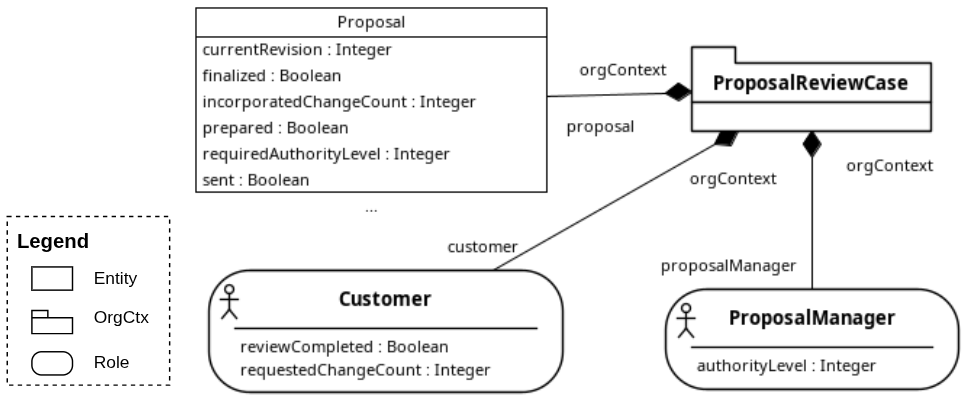
\includegraphics[width=\columnwidth,keepaspectratio]{images/ACLmodel.png}
\vspace{-1.1em}
\begin{center}
\caption{ACL model of \textit{MeetingScheduler}.}
\label{fig:acl-mtg}
\end{center}
\vspace{-2.7em}
\end{center}
\end{figure}

%%%%%%%%%%%%%%%%%%%%%%%%%%%%%%%%%%%%%%%%%%%%%%%%%%%%%
\subsection{The Simplified BPMN Language}
\label{sec:bpmn}
\label{sec:bpmn-semantics}
%%%%%%%%%%%%%%%%%%%%%%%%%%%%%%%%%%%%%%%%%%%%%%%%%%%%%

The simplified BPMN language gives operational semantics to the process view. It retains pools, lanes, activities, start and end events, sequence flows, and exclusive, inclusive, and parallel gateways from BPMN~\cite{omg2013bpmn} (Figure~\ref{fig:bpmn-metamodel}). A pool is typed by an ACL group and denotes one process instance for each matching group occurrence; a lane is typed by an ACL role, and an activity executed in that lane must be performed by an agent playing the corresponding role in the pool's group occurrence.

\begin{figure}[htbp]
\vspace{-.3em}
\begin{center}
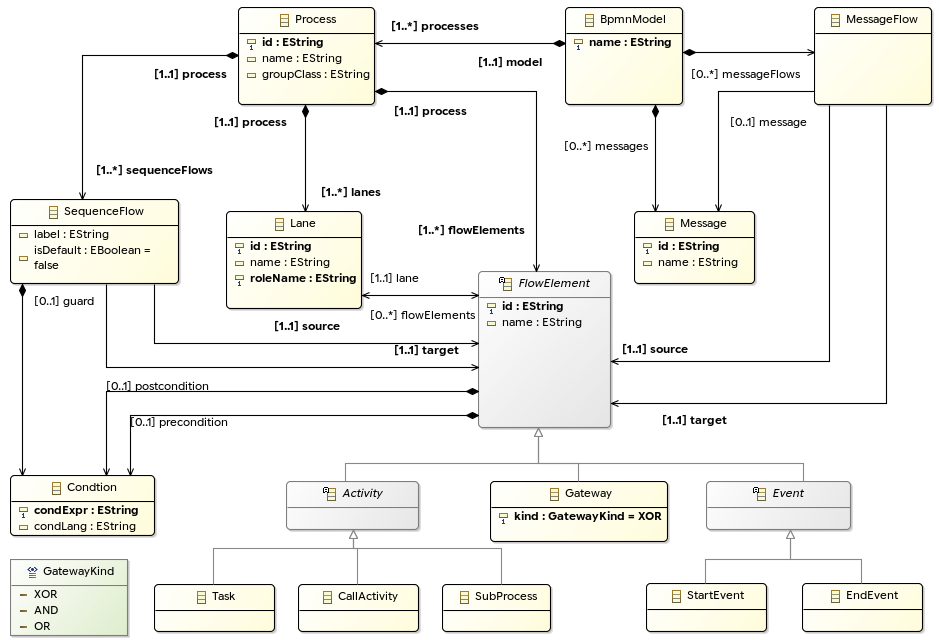
\includegraphics[width=\columnwidth,keepaspectratio]{images/BPMNMetamodel.png}
\vspace{-1.1em}
\begin{center}
\caption{The simplified BPMN metamodel.}
\label{fig:bpmn-metamodel}
\end{center}
\vspace{-2.7em}
\end{center}
\end{figure}

\begin{definition}[BPMN Process State]
\label{def:bpmn-model}
A BPMN process is $B=(T,F)$, where $T=E\uplus A\uplus G_B$ partitions its flow nodes into start/end events, activities, and gateways, and $F\subseteq T\times T$ is the sequence-flow relation. Writing $F_B=F\cup\{(\bot,s)\mid s\text{ a start event}\}$ for the flow domain extended with a process-entry symbol $\bot$, a control state is a set of active flows $\sigma_F\subseteq F_B$, initially the entry flows of every start event. Executing an active flow $f$ transitions
\[
\sigma_F \xrightarrow{\mathit{target}(f)}_B \sigma_F': \quad \sigma_F' = (\sigma_F\setminus \mathit{Pass}(f)) \cup \mathit{Next}(f),
\]
where $\mathit{Pass}(f)$ and $\mathit{Next}(f)$ specialize by node type: an activity or a start/end event consumes just $f$ and, unless it is an end event, produces every outgoing flow; an exclusive gateway consumes $f$ and produces exactly one outgoing flow; an inclusive gateway consumes and produces non-empty subsets of, respectively, its incoming and outgoing flows; and a parallel gateway consumes all incoming flows and produces all outgoing flows. A configuration is final when every active flow targets an end event.
\end{definition}

Activities additionally carry an OCL precondition and, per outgoing flow, a branch-specific postcondition over ACL: a precondition determines whether the activity's execution is enabled, and a postcondition relates the ACL state before execution to the state after it. Gateways change only the control configuration $\sigma_F$; how activity execution is checked and applied against the shared ACL state is given uniformly, together with the other node types, in Section~\ref{sec:checking}.

Figure~\ref{fig:bpmn-mtg} instantiates this language with one pool for a meeting unit and lanes for its initiator, organizer, secretary, and participants. The initial activities decide the meeting details; an exclusive gateway selects calendar collection or telephone contact according to ACL data; subsequent activities choose a time, notify the participants, and record attendance. The process thereby generates the ACL state changes over which the i* model of Section~\ref{sec:istar} is evaluated.

%%%%%%%%%%%%%%%%%%%%%%%%%%%%%%%%%%%%%%%%%%%%%%%%%%%%%
\subsection{The Extended i* Language}
\label{sec:istar}
%%%%%%%%%%%%%%%%%%%%%%%%%%%%%%%%%%%%%%%%%%%%%%%%%%%%%

The extended i* language specifies intentions over ACL states. Its metamodel (Figure~\ref{fig:istar-metamodel}) retains actors, goals, tasks, resources, qualities, obstacles, refinements, contributions, and strategic dependencies from i*~\cite{yu1997towards}. An actor is typed by an ACL role, so one actor definition induces one intentional-element instance for every matching role occurrence in a concrete ACL population, rather than a single model-level truth value. Goals carry a temporal kind---\texttt{Achieve}, \texttt{Maintain}, \texttt{Sustain}, or \texttt{Recur} (repeated \texttt{Achieve})---and an OCL \texttt{condition}; tasks carry OCL pre/postconditions. Two quantified refinements support this instance-level reasoning: a \texttt{forall} refinement creates a child context for every matching role occurrence and aggregates all of them, while a \texttt{pick} refinement selects one matching occurrence and keeps that choice stable across checkpoints; an empty quantified domain yields an unknown result rather than vacuous satisfaction. Strategic dependencies transfer the evaluation context from a depender occurrence to a matching dependee occurrence.

\begin{figure}[htbp]
\vspace{-.3em}
\begin{center}

\includegraphics[width=\columnwidth,keepaspectratio]{images/IstarMetamodel.png}
\vspace{-1.1em}
\begin{center}
\caption{The extended i* metamodel.}
\label{fig:istar-metamodel}
\end{center}
\vspace{-2.7em}
\end{center}
\end{figure}

\begin{definition}[Instance-Level Goal Marking]
\label{def:goal-marking}
An i* actor is typed by an ACL role $a$; its runtime instances at checkpoint $i$ are the occurrences $\sigma_{\mathit{Class}}^i(a)$, and $g^x$ denotes the instance of goal $g$ bound to occurrence $x$. Its state condition is
\[
\mathit{eval}_{\sigma_M^i}(g^x)=\top \iff \mathit{condition}(g)\text{ holds for }x\text{ in }\sigma_M^i,
\]
and its marking $\mathit{evalGoal}_i(g^x)\in\Delta=\{(?,?),(\top,\bot),(\top,\top)\}$---respectively undetermined, activated but unfulfilled, and fulfilled---follows its temporal kind:
\[
\mathit{evalGoal}_i(g^x)=
\begin{cases}
(\top,\top), & \mathit{eval}_{\sigma_M^i}(g^x)=\top,\\
(\top,\bot), & \mathit{eval}_{\sigma_M^i}(g^x)=\bot,
\end{cases}
\]
for a \texttt{Maintain} goal;
\[
\mathit{evalGoal}_i(g^x)=
\begin{cases}
(\top,\top), & \mathit{evalGoal}_{i-1}(g^x)=(\top,\top) \text{ or } \mathit{eval}_{\sigma_M^i}(g^x)=\top,\\
(?,?), & \text{otherwise},
\end{cases}
\]
for an \texttt{Achieve} goal, so that fulfillment latches; and, for a \texttt{Sustain} goal, as \texttt{Achieve} until first fulfilled, after which a later violation of $\mathit{eval}_{\sigma_M^i}$ yields $(\top,\bot)$, which then persists as under \texttt{Maintain}. A non-leaf goal or task carries no directly attached condition and is evaluated exclusively from its AND/OR-, \texttt{forall}-, or \texttt{pick}-refined children, so a parent marking never bypasses or contradicts them; task, quality, obstacle, and dependency markings are derived analogously, from their own preconditions, postconditions, and incoming contribution or obstruction links.
\end{definition}

In Figure~\ref{fig:istar-mtg}, \texttt{MeetingOrganized} is evaluated for the concrete initiator occurrence. Its scheduling branch is delegated to an organizer, while its attendance branch uses \texttt{forall} over the participant occurrences owned by the same meeting unit. Timetable collection may use an OR between calendar and telephone channels, and a \texttt{pick} identifies the secretary occurrence that performs the call. Hence the same i* model can distinguish a meeting in which all participants attend from one in which only one of several participants is reached.

%%%%%%%%%%%%%%%%%%%%%%%%%%%%%%%%%%%%%%%%%%%%%%%%%%%%%
\subsection{Transformation to Event-B}
\label{sec:eventb-transformation}
%%%%%%%%%%%%%%%%%%%%%%%%%%%%%%%%%%%%%%%%%%%%%%%%%%%%%

The transformation $\mathcal T(\mathcal A,I,B)$ produces an Event-B context containing static domains and a machine containing the integrated dynamic state. The rules are compositional and preserve the bindings established among the source models.

\emph{ACL rules.} Each root entity/group identity domain and each role occurrence domain becomes a carrier set; ordinary entity/group specializations reuse their parent's domain, and enumerations become finite partitions. Current extents, properties, associations, containment links, and play relations become machine variables. Their typing, multiplicity, generalization, containment, role-chain, and compatibility conditions become invariants, and all dynamic extents and relations are initialized to the empty set. This encoding is the basis of Definition~\ref{def:acl-model}.

\emph{BPMN rules.} A pool introduces process-instance and lifecycle variables together with a scope function from each process instance to its ACL group occurrence. Every sequence flow becomes a token-count function indexed by process instance. Start, activity, gateway, and end nodes become Event-B events. An activity event is guarded by its input token, lane-role binding, and translated OCL precondition; its simultaneous actions update the token functions and ACL variables according to the postcondition. Exclusive, inclusive, and parallel gateways are translated into guarded branch, split, merge, and join events.

\emph{i* rules.} i* actors reuse the ACL role extents rather than introducing duplicate actor populations. Goal and task occurrences, context bindings, and marking components become machine variables. Activation and condition expressions become predicates, while AND, OR, \texttt{forall}, \texttt{pick}, contribution, obstruction, and dependency relations determine the marking-update actions. Quantified refinements range over the current ACL role occurrences in the required group context.

\emph{Synchronization rule.} The integrated machine has phases \texttt{READY} and \texttt{DIRTY}. Every translated BPMN step moves the machine from \texttt{READY} to \texttt{DIRTY}. The event \texttt{EvaluateAllGoals} then evaluates the entire i* model atomically and returns it to \texttt{READY}; only such states are observable checkpoints. Rodin generates well-definedness and invariant-preservation obligations for these events, so the proof concerns the integrated semantics rather than three unrelated translations. This follows the established use of Event-B for formal BPMN analysis~\cite{bryans2010eventb}, extended here with ACL state and i* markings.

%%%%%%%%%%%%%%%%%%%%%%%%%%%%%%%%%%%%%%%%%%%%%%%%%%%%%
\subsection{Synchronization and Conformance}
\label{sec:checking}
%%%%%%%%%%%%%%%%%%%%%%%%%%%%%%%%%%%%%%%%%%%%%%%%%%%%%

The definitions above give each language its own state: ACL contributes the domain and organizational state $\sigma_M$, BPMN the control state $\sigma_F$, and i* a marking derived from $\sigma_M$ at every checkpoint (Definition~\ref{def:goal-marking}). Conformance checking aligns these along one concrete execution.

\begin{definition}[Synchronized Step]
\label{def:synchronized-transition}
Let $f$ be a BPMN flow, with precondition $\mathit{Pre}_B(f)$ taken from its target activity (or $\top$ if its target is not an activity) and branch postcondition $\mathit{Post}_B(f)$ taken from its source. Executing $f$ as step $i$ is a synchronized step
\[
\langle\sigma_F^{i-1},\sigma_M^{i-1}\rangle \xRightarrow{f}\langle\sigma_F^i,\sigma_M^i\rangle
\]
iff (a) $\sigma_F^{i-1}\xrightarrow{\mathit{target}(f)}_B\sigma_F^i$ (Definition~\ref{def:bpmn-model}), (b) $\sigma_M^{i-1}\models\mathit{Pre}_B(f)$, (c) $(\sigma_M^{i-1},\sigma_M^i)\models\mathit{Post}_B(f)$, and (d) $\sigma_M^i\models\mathit{Inv}(\mathcal A)$.
\end{definition}

Condition (a) is a purely BPMN control-flow step; conditions (b)--(d) tie that step to the shared ACL state and, being OCL, are declarative rather than constructive: (b) constrains the state in which $f$ may execute, (c) constrains the relationship between the two consecutive ACL states, and (d) constrains every admissible state. A step whose control flow is possible but whose associated domain-state change is not licensed by (b)--(d) is rejected. Every resulting $\sigma_M^i$ is a new checkpoint at which the i* marking is reevaluated (Definition~\ref{def:goal-marking}), so a BPMN execution step is related to its effect on intentional satisfaction without introducing a separate state representation for the goal model.

\begin{definition}[Scenario Conformance]
\label{def:conformance}
A scenario is $S=(\mathcal A,I,B,\sigma_M^0,\tau,\mathcal O)$, where $\sigma_M^0$ is an AOL-derived initial ACL state, $\tau=\langle f_1,\ldots,f_n\rangle$ is a concrete BPMN execution with its process-instance and role bindings, and $\mathcal O$ is an optional oracle of expected i* markings. Replaying $\tau$ from $(\sigma_F^0,\sigma_M^0)$ through repeated synchronized steps yields a checkpoint trace and, by Definition~\ref{def:goal-marking}, a marking trace $\langle M_0,\ldots,M_n\rangle$. Writing $G_{\mathit{root}}^n$ for the instantiated root-goal occurrences present at the final checkpoint, the scenario conforms iff
\begin{align*}
\mathit{Conform}(S)\iff{}&
\textstyle\bigwedge_{i=1}^n\langle\sigma_F^{i-1},\sigma_M^{i-1}\rangle\xRightarrow{f_i}\langle\sigma_F^i,\sigma_M^i\rangle\\
&{}\land\ \mathit{Final}_B(\sigma_F^n)\\
&{}\land\ \forall g^x\in G_{\mathit{root}}^n:\ \mathit{evalGoal}_n(g^x)=(\top,\top)\\
&{}\land\ \mathit{Agree}(M_n,\mathcal O),
\end{align*}
where the last conjunct is omitted when no oracle is supplied.
\end{definition}

The four conjuncts are diagnostically distinct. The first requires every replayed step to be a valid synchronized step, so a violated ACL invariant, an unmet precondition, or a falsified postcondition each break the chain at the checkpoint where it occurs. The second requires the BPMN execution to reach a final configuration: a process may execute all of its activities and terminate normally while still producing a state that does not satisfy the intentions it is expected to serve, which is why process completion alone does not establish conformance. The third is instance-quantified: because $G_{\mathit{root}}^n$ ranges over root-goal \emph{instances} rather than model-level goals, a scenario is not conformant merely because some instance of a root goal is satisfied---every relevant instance present at the final checkpoint must be, so that a satisfied participant cannot mask a violation concerning another participant represented by the same model-level goal. The last conjunct compares the computed marking trace against the supplied oracle, when one is given. The checker reports these four possibilities separately, as \texttt{aclFailures}, \texttt{bpmnFailures}, \texttt{goalFailures}, and \texttt{oracleFailures}, so a failed verdict identifies both the first divergent checkpoint and the responsible model (Section~\ref{sect:discussion}). The notion is deliberately scenario-based: it establishes conformance for the analyzed execution $\tau$, not a universal property over every trace reachable from the BPMN model; paths and instance populations not represented by the scenario are outside its claim.



%%%%%%%%%%%%%%%%%%%%%%%%%%%%%%%%%%%%%%%%%%%%%%
\section{Tool Support}
\label{sect:toolSupport}
%%%%%%%%%%%%%%%%%%%%%%%%%%%%%%%%%%%%%%%%%%%%%%

We implemented the proposed approach as a prototype, called the \textit{Goal Plugin}, to support the model transformation and verification workflow. The plugin takes three source models---ACL, iStar, and BPMN---and translates them into a unified Event-B project for verification in Rodin. These models capture complementary system perspectives: ACL specifies the structural state space, BPMN defines the behavioral transitions, and iStar captures the intentional requirements.

Each source model is processed by a dedicated translator that generates a corresponding Event-B fragment. The ACL translator produces the structural elements, including carrier sets, variables, relations, invariants, and initialization actions. The BPMN translator maps process elements to Event-B events and translates their guards and effects into Event-B guards and actions. While the iStar translator generates the intentional elements required to represent and evaluate goal and task satisfaction.

The generated fragments are then composed into a single Event-B model. In the resulting composition, ACL defines the admissible state space, BPMN defines the transition system over that state space, and iStar provides the goal-satisfaction layer. The plugin generates a Rodin-compatible project containing the corresponding Event-B contexts, machines, events, invariants, and traceability information linking generated elements to their source models.

Rodin serves as the verification backend, where the generated Event-B model is analysed through proof obligations to establish the consistency of the integrated structural, behavioral, and intentional specifications. The meeting-scheduling case study is used to demonstrate the complete tool-supported workflow, from source-model translation and composition to formal verification of the resulting Event-B model.

Figure~\ref{fig:tool} illustrates the overall architecture of the Goal Plugin and its integration with the model transformation and verification workflow. It shows how the three source models are independently translated into Event-B fragments, composed into a unified Event-B project, and subsequently verified using Rodin.

\begin{figure}[htbp]
\vspace{-.3em}
\begin{center}
\includegraphics[width=\columnwidth,keepaspectratio]{images/ToolSupport.png}
\vspace{-1.1em}
\begin{center}
\caption{Architecture of the \textbf{Goal Plugin}.}
\label{fig:tool}
\end{center}
\vspace{-2.7em}
\end{center}
\end{figure}

%%%%%%%%%%%%%%%%%%%%%%%%%%%%%%%%%%%%%%%%%%%%%%%%%%%%%%%%%%%%%
\section{Evaluation}
\label{sect:evaluative}
%%%%%%%%%%%%%%%%%%%%%%%%%%%%%%%%%%%%%%%%%%%%%%%%%%%%%%%%%%%%%

The evaluation is organized around two research questions:
\begin{itemize}
  \item \textbf{RQ1.} How can the organizational structure of a system be formally specified during analysis alongside its goal and process models?
  \item \textbf{RQ2.} How can the evolving states of a goal model and a process model be represented in a shared intermediate model so that their consistency can be checked along a concrete execution scenario?
\end{itemize}

RQ1 is addressed by the ACL, simplified BPMN, and extended i* metamodels (Sections~\ref{sec:acl-language}, \ref{sec:bpmn}, and~\ref{sec:istar}). RQ2 is addressed by the state-transition semantics and checking algorithm (Sections~\ref{sec:bpmn-semantics}, \ref{sec:eventb-transformation}, and~\ref{sec:checking}) and the tool of Section~\ref{sect:toolSupport}. The rest of this section positions these answers against three representative techniques.

GoBIS~\cite{gobis2015} provides integration guidelines and traceability between goal and process perspectives, but operates at design time. Gr\"oner et al.'s~\cite{groner2014vadl} Description-Logic approach automatically validates mappings between intentional relations and process structures, but does not represent execution order. Caballero-Villalobos et al.~\cite{caballero2026alig} provide the strongest behavioral guarantee, a verdict over every reachable execution rather than one trace; this method instead evaluates one concrete scenario over the actor and domain instances represented in the shared USE/OCL state.

None of the three would catch the \texttt{pick}/\texttt{forall} case of Section~\ref{sec:checking} on \textit{MeetingScheduler}, where one participant is never reached although every executed activity and every other participant's marking checks out. Their goal markings are not instance-quantified, so a \texttt{pick}-satisfied sub-goal and an OR-satisfied sibling can be sufficient to mark the model-level goal as satisfied, with no way to expose the omitted instance. The proposed method adds this instance-level checking over a shared state, at the cost of checking one concrete trace instead of every reachable execution (Section~\ref{sect:discussion}).

%%%%%%%%%%%%%%%%%%%%%%%%%%%%%%%%%%%%%%%%%%%%%%%%%%%%%%%%%%%%%
\section{Discussion}
\label{sect:discussion}
%%%%%%%%%%%%%%%%%%%%%%%%%%%%%%%%%%%%%%%%%%%%%%%%%%%%%%%%%%%%%

\subsection{Separating four kinds of failure}
Splitting the result into \texttt{aclFailures}, \texttt{bpmnFailures}, \texttt{goalFailures}, and \texttt{oracleFailures}, rather than one verdict, separates failures of the shared state from failures of process execution, goal realization, and expected markings. This separation is diagnostically useful because each category points to a different source artifact. When one checkpoint violates more than one category, the current implementation reports ACL invariants before BPMN pre/postconditions as an implementation order, not as a statement of business priority.

\subsection{One trace, not every trace}
Checking one concrete scenario answers whether that scenario is consistent, not whether every scenario is, the stronger guarantee that weak/strong compliance in Caballero-Villalobos et al.~\cite{caballero2026alig} gives for the goal--process pair alone. This is deliberate: it trades that generality for running immediately on the existing USE/OCL execution environment. Because the checker takes the scenario as an ordinary parameter, the pipeline can be re-run over several scenarios to raise coverage, though without the same formal guarantee as full state-space exploration.

\subsection{Limitations}
\emph{Coverage.} Gateway guards resolve one execution for the supplied scenario, so branches not selected in that execution are not exercised; a \texttt{PASS} is a statement about the trace checked, not every trace. \emph{Scenario quality.} An under-populated AOL snapshot can let the root-goal check skip actors absent from the scenario. \emph{Fail-fast masking.} A second ACL violation occurring after the first may only surface on a subsequent run. \emph{Evaluation scope.} The evidence rests on two case studies; broader validation and a running-time measurement are left for future work.

%%%%%%%%%%%%%%%%%%%%%%%%%%%%%%%%%%%%%%%%%%%%%%%%%%
\section{Related work}
\label{sect:relatedWork}
%%%%%%%%%%%%%%%%%%%%%%%%%%%%%%%%%%%%%%%%%%%%%%%%%%

% A first line of work integrates goal and process models at design time. GoBIS~\cite{gobis2015} combines i* and Communication Analysis through a metamodel integration and methodological guidelines, improving traceability and model completeness. Gr\"oner et al.~\cite{groner2014vadl} formalize mappings between goal relations and process structures in Description Logics and automatically detect orchestration and choreography inconsistencies. These approaches validate the models and their correspondences as specified, rather than goal satisfaction along a concrete execution.

% A second line of work evaluates behavioral consistency. Our previous work~\cite{dang2010jucs} synchronizes two scenarios through a common conceptual model and OCL, establishing consistency along one execution. Caballero-Villalobos et al.~\cite{caballero2026alig} translate goal and process models into transition systems and decide weak, strong, and monotonic compliance over reachable executions. The former is limited to the scenario examined, while the latter provides broader behavioral guarantees but still relates executions to model-level intentional elements.

% Formal verification has also been applied to process models independently of their goal models. Bryans and Wei~\cite{bryans2010eventb} give an algorithmic translation of BPMN control and data flow into Event-B for verification with Rodin. Our transformation instead covers the integrated ACL, goal, and process specifications, preserving the shared state used for consistency checking.

% Across these lines of work, correspondence is primarily established between model-level elements or states. The proposed method instead evaluates both process effects and quantified goal satisfaction over the same actor and domain instances. ACL structural invariants are checked on that state as an additional validation layer, but the central consistency claim remains whether the process-generated state realizes the applicable goals.

Existing research on the relationship between goal and process models can be broadly organized into three areas: structural consistency checking, execution-based consistency checking, and goal--process integration.

\textit{Structural consistency checking.}
Gr\"oner et al.~\cite{groner2014vadl} formalize correspondences between intentional relations and process structures using Description Logics, enabling automated detection of inconsistencies in process orchestration and choreography. Such approaches primarily reason about model-level elements and their relationships, rather than the states resulting from a concrete process execution.

\textit{Execution-based consistency checking.}
Dang et al.~\cite{dang2010jucs} synchronize execution scenarios through a common conceptual model and use OCL constraints to assess conformance along a trace. Caballero-Villalobos et al.~\cite{caballero2026alig} adopt a broader behavioral perspective by translating goal and process models into transition systems and evaluating compliance over reachable executions. Our approach remains scenario-based, but evaluates goal satisfaction over the same instance-level ACL states modified during BPMN execution. Related work on formal process verification translates BPMN into Event-B for analysis with Rodin~\cite{bryans2010eventb}; in our approach, the transformation instead covers the integrated ACL, i*, and BPMN semantics.

\textit{Goal--process integration.}
Koliadis and Ghose~\cite{koliadis2006goalbpm} relate BPMN process models to KAOS goals through the GoalBPM methodology. In related work, Koliadis et al.~\cite{koliadis2006ibpmn} combine i* and BPMN to support business process model lifecycle management through fulfillment conditions and process activity effects. GoBIS~\cite{gobis2015} integrates i* and Communication Analysis through metamodel integration and methodological guidelines, while URN combines goal and scenario modelling within an integrated framework~\cite{amyot2022combining}. In contrast, our approach retains separate goal and process models and introduces ACL as a shared state model through which BPMN execution effects and i* intentions are related.

Overall, our approach differs from existing work by checking consistency over concrete organizational and domain instances represented in the shared state. This makes it possible to identify executions in which the process completes, while a goal remains unsatisfied for a specific actor or role instance. However, the result is limited to the examined execution scenario rather than all possible executions.


%%%%%%%%%%%%%%%%%%%%%%%%%%%%%%%%%%%%%%%%%%%%%%
\section{Conclusion}
\label{sect:conclusion}
%%%%%%%%%%%%%%%%%%%%%%%%%%%%%%%%%%%%%%%%%%%%%%

This paper has presented a shared-state methodology for checking consistency between goal and process models. Its first contribution is ACL, which makes the organizational and domain state shared by the two views explicit. Its second contribution is an extended state-based semantics for i* and a simplified operational semantics for BPMN, connected through checkpoint traces over the same ACL state. Third, systematic transformation rules map the integrated ACL, i*, and BPMN specifications to Event-B, enabling Rodin to perform static checking and discharge proof obligations concerning typing and safety. Fourth, a plugin integrated into the USE environment realizes the scenario-based method through batch checking and step-by-step visual debugging.

Through the \textit{MeetingScheduler} case study, the method exposes an instance-level divergence in which the BPMN execution completes although an applicable i* goal remains unsatisfied for one participant. The incident-response case study provides additional evidence that the same pipeline applies to a distinct process scenario. As discussed in Section~\ref{sect:discussion}, the method checks a single concrete execution trace rather than every reachable one. Future work includes re-running the pipeline over multiple scenarios to increase coverage, exploring the reachable state space, and conducting a broader empirical evaluation with running-time measurements as scenario size grows.

%%%%%%%%%%%%%%%%%%%%%%%%%%%%%%%%%%%%%%%%%%%%%%
\balance
%\vspace{-0.5em}
\bibliographystyle{IEEEtran}
\bibliography{references}
\end{document}
